\documentclass{report}
\usepackage{graphicx}

\begin{document}

\begin{titlepage}
    \centering
    
\includegraphics[width=0.3\textwidth]{logo.jpg}\par\vspace{1cm}
    {\scshape\Large Université Des Antilles \par}
    \vspace{1cm}
    {\scshape\Large Master Mathématiques et Applications \par}
    \vspace{3cm}
    {\huge\bfseries Titre de votre mémoire \par}
    \vspace{3cm}
    {\Large\itshape Votre Nom \par}
    \vfill
    Supervisé par\par
    Nom de l'Encadreur

    \vfill

    % Bottom of the page
    {\large \today\par}
\end{titlepage}

\chapter*{Remerciements}
\addcontentsline{toc}{chapter}{Remerciements}

Insérez remerciements ici.

\tableofcontents
\newpage

\chapter*{Introduction}
\addcontentsline{toc}{chapter}{Introduction}

La Martinique, île des Caraïbes réputée pour sa biodiversité et son agriculture, est confrontée depuis plusieurs décennies à un problème environnemental majeur : la contamination des sols agricoles par le chlordécone. Utilisé massivement dans les plantations de bananes entre les années 1970 et 1993, le chlordécone, pesticide organochloré persistant, persiste dans l'environnement et représente une menace pour la santé publique et la sécurité alimentaire.

La dégradation du chlordécone dans les sols agricoles est un processus complexe influencé par une multitude de facteurs environnementaux. Comprendre ces facteurs et leur interaction est essentiel pour élaborer des stratégies efficaces de gestion et de décontamination des terres agricoles martiniquaises.

La présente étude se propose d'explorer en profondeur cette problématique en se concentrant sur les principaux facteurs environnementaux qui influencent la dégradation du chlordécone dans les sols agricoles de la Martinique sur une période de 15 ans. Plus précisément, nous chercherons à répondre à la question suivante : quels sont les facteurs environnementaux qui interagissent pour influencer la dégradation du chlordécone, et comment ces interactions affectent-elles ce processus au fil du temps ?

Pour répondre à cette question, nous adopterons une approche multidisciplinaire, combinant des analyses statistiques avancées, des techniques de modélisation environnementale et une exploration approfondie des données longitudinales sur les niveaux de chlordécone et les variables environnementales pertinentes. Cette approche nous permettra d'identifier les tendances principales, de caractériser les facteurs environnementaux clés et d'évaluer leur impact sur la dégradation du chlordécone dans les sols agricoles martiniquaises.

En fin de compte, cette recherche vise à enrichir notre compréhension des processus de dégradation du chlordécone dans un contexte insulaire et tropical, et à fournir des connaissances fondamentales pour orienter les politiques de gestion environnementale et les pratiques agricoles durables dans la région de la Martinique.

\chapter*{État des connaissances sur la dégradation du chlordécone dans les sols agricoles martiniquais.}
\addcontentsline{toc}{chapter}{État des connaissances sur la dégradation du chlordécone dans les sols agricoles martiniquais.}

\section{Effets du chlordécone sur l'environnement et la santé humaine}
\addcontentsline{toc}{section}{Effets du chlordécone sur l'environnement et la santé humaine}
Le chlordécone, un pesticide organochloré largement utilisé dans les plantations de bananes en Martinique jusqu'au début des années 1990, est connu pour ses effets néfastes sur l'environnement et la santé humaine. Des études ont montré sa persistance dans les sols agricoles, son accumulation dans la chaîne alimentaire et son association avec des risques pour la santé, notamment des effets neurotoxiques et cancérigènes chez l'homme.

\section{Processus de dégradation du chlordécone}


La dégradation du chlordécone dans les sols agricoles est un processus complexe influencé par divers facteurs environnementaux. Les études précédentes ont identifié plusieurs voies de dégradation, notamment la biodégradation par des microorganismes du sol, l'adsorption sur les particules du sol et la dégradation photochimique sous l'effet de la lumière solaire. Cependant, la compréhension de ces processus reste incomplète, en particulier en ce qui concerne leur cinétique et leurs mécanismes exacts.

\section{Facteurs environnementaux influençant la dégradation du chlordécone}


Plusieurs études ont examiné l'impact des facteurs environnementaux sur la dégradation du chlordécone dans les sols agricoles. Ces facteurs comprennent le type de sol, l'exposition solaire, la température, l'humidité du sol, le pH du sol et la présence de microorganismes dégradateurs. Cependant, les résultats de ces études sont parfois contradictoires, ce qui souligne la nécessité d'une analyse approfondie et intégrée des facteurs environnementaux pour comprendre pleinement leur rôle dans le processus de dégradation du chlordécone.

\section{Lacunes}


Malgré les progrès réalisés dans la compréhension de la dégradation du chlordécone, plusieurs lacunes subsistent. Ces lacunes incluent le manque de données longitudinales à long terme sur la dégradation du chlordécone dans les sols agricoles de la Martinique, ainsi que l'absence d'études intégrant de manière exhaustive les différents facteurs environnementaux influençant ce processus.
\\

Dans cette section,on met en évidence l'importance cruciale de comprendre les processus de dégradation du chlordécone dans les sols agricoles martiniquaises, ainsi que les facteurs environnementaux qui les influencent. Cette compréhension est essentielle pour élaborer des stratégies efficaces de gestion et de décontamination des terres agricoles contaminées par le chlordécone dans la région de la Martinique.



\chapter*{Méthodologie}
\addcontentsline{toc}{chapter}{Méthodologie}


La méthodologie adoptée dans cette étude est cruciale pour répondre à la problématique posée et atteindre les objectifs fixés. Cette section détaille les données utilisées, les méthodes analytiques appliquées et les étapes suivies pour mener à bien l'analyse des facteurs environnementaux influençant la dégradation du chlordécone dans les sols agricoles de la Martinique sur une période de 15 ans.

\section{Données utilisées}
\addcontentsline{toc}{section}{Données utilisées}

Les données utilisées dans cette étude ont été fournies par le Dr Zongo Pascal, Docteur en mathématiques et professeur à l'Université des Antilles. Elles sont constituées de deux fichiers au format CSV : l'un contenant les données brutes et l'autre contenant les explications sur la signification des données et les définitions des colonnes.

Le fichier de données brutes comprend une série temporelle détaillée des niveaux de chlordécone dans les sols agricoles de la Martinique sur une période de 15 ans, de 2004 à 2019. Chaque entrée dans ce fichier représente un échantillon de sol prélevé à un emplacement spécifique, avec des mesures de concentration de chlordécone ainsi que des variables environnementales telles que la pluviométrie, l'exposition solaire, la rugosité du terrain, etc.

Le deuxième fichier fournit des explications sur la signification de chaque variable présente dans le fichier de données brutes, ainsi que des définitions des colonnes. Ces informations sont essentielles pour comprendre et interpréter correctement les données, en particulier pour identifier les facteurs environnementaux pertinents qui pourraient influencer la dégradation du chlordécone dans les sols agricoles de la Martinique.
 
\section{Méthodes analytiques}

Pour analyser les données longitudinales sur les niveaux de chlordécone et les variables environnementales, plusieurs méthodes analytiques ont été utilisées. Tout d'abord, une analyse statistique descriptive a été réalisée pour explorer les tendances temporelles et spatiales des concentrations de chlordécone dans les sols agricoles de la Martinique. Ensuite, des modèles statistiques adaptés aux données longitudinales ont été appliqués pour évaluer l'impact des facteurs environnementaux sur la dégradation du chlordécone. Ces modèles ont permis de prendre en compte la structure temporelle des données et les interactions entre les différentes variables.

En outre, des techniques de clustering et de classification dynamique ont été employées pour regrouper les parcelles en fonction de leur profil de décontamination du chlordécone. Ces techniques ont permis d'identifier des groupes de terres présentant des caractéristiques similaires en termes de vitesse et de pattern de dégradation du chlordécone, ce qui a facilité la caractérisation des différents profils de décontamination.
\\

 \section{Logiciel et Packages Utilisés}
 Dans cette étude, nous avons utilisé le langage de programmation R pour la manipulation des données, l'analyse statistique, et la modélisation. R est un langage puissant et flexible, particulièrement adapté pour les analyses de données complexes et les visualisations. Les packages spécifiques utilisés dans cette étude sont décrits ci-dessous :\\
 
corrplot : Créer des graphiques de corrélation pour mieux comprendre les relations entre les variables.\\
  
dplyr : Fournit des outils pour manipuler les données de manière efficace.\\

nlme : Ce package permet de réaliser des modèles linéaires mixtes. Ces modèles sont utiles pour analyser les données avec des structures de corrélation et de variabilité complexes, en tenant compte des effets fixes et aléatoires.\\

lme4 : Un package similaire à nlme, utilisé pour ajuster des modèles linéaires et non linéaires avec effets mixtes. Il est particulièrement performant pour les grands ensembles de données.\\

kmeans : Fonction de base dans R utilisée pour effectuer une analyse de clustering en utilisant l'algorithme K-means. Cet algorithme permet de regrouper les parcelles en fonction de leurs caractéristiques similaires.\\

dtwclust : Ce package permet la réalisation de clustering sur des séries temporelles en utilisant des distances dynamiques de type DTW (Dynamic Time Warping), utile pour analyser les profils de dégradation au fil du temps.\\

ggplot2 : Un package de visualisation de données basé sur la grammaire des graphiques. Il permet de créer des visualisations élégantes et complexes de manière simple et intuitive.\\

reshape2 : Utilisé pour réorganiser les données (par exemple, pour passer d'un format large à un format long), facilitant ainsi l'analyse et la visualisation.
\\
En plus de R, nous avons également utilisé Power BI, un outil puissant de business intelligence et de visualisation de données. Power BI nous a permis de créer des tableaux de bord interactifs et des graphiques dynamiques pour explorer et présenter les résultats de manière claire et intuitive.
\\
\section{Stratégies d'évaluation des résultats}

Dans cette section, nous examinerons les stratégies utilisées pour évaluer les résultats de notre étude sur la dégradation du chlordécone dans les sols agricoles de la Martinique. Les stratégies d'évaluation comprennent généralement une combinaison de mesures quantitatives et qualitatives pour évaluer la pertinence et la fiabilité des résultats obtenus. Voici quelques stratégies clés que nous pourrions utiliser :

Analyse des tendances temporelles \\
   - Nous analyserons les tendances temporelles des niveaux de chlordécone dans les sols agricoles au fil des années pour identifier toute évolution significative dans la dégradation du chlordécone. Cela pourrait inclure l'utilisation de graphiques de séries chronologiques pour visualiser les changements au fil du temps.

Analyse des corrélations\\
   - Nous examinerons les corrélations entre les niveaux de chlordécone et les variables environnementales telles que la pluviométrie, l'ensoleillement, la rugosité du terrain, etc. Cela nous aidera à déterminer les facteurs qui influencent le processus de dégradation du chlordécone.


Analyse de la variabilité inter-parcelles
   - Nous évaluerons la variabilité des taux de dégradation du chlordécone entre différentes parcelles agricoles. Cela peut être réalisé en calculant les écarts-types des taux de dégradation ou en utilisant des techniques d'analyse de variance (ANOVA) pour comparer les moyennes entre les parcelles.

Validation des clusters et des classifications
   - Si nous avons utilisé des techniques de clustering ou de classification pour regrouper les parcelles en fonction de leurs profils de dégradation, nous évaluerons la validité de ces groupes en utilisant des mesures telles que l'indice de Davies-Bouldin ou l'indice de silhouette. Cela nous aidera à déterminer la cohérence et la qualité des regroupements obtenus.

Analyse de sensibilité
   - Nous effectuerons une analyse de sensibilité pour évaluer la robustesse de nos résultats par rapport à différentes hypothèses ou paramètres utilisés dans notre analyse. Cela nous permettra de déterminer la stabilité de nos conclusions face à des variations potentielles dans les méthodes ou les données utilisées.

Consultation des documents\\
   - Enfin, nous pourrions consulter des documents du ministère de la Santé publique ,les études et les publications publiés par le ministère de la Santé publique de la Martinique. Ces documents peuvent contenir des informations précieuses sur la contamination par le chlordécone, ses effets sur la santé publique et les efforts de gestion de cette pollution..

En utilisant une combinaison de ces stratégies, nous serons en mesure d'évaluer de manière approfondie les résultats de notre étude sur la dégradation du chlordécone dans les sols agricoles de la Martinique. Cela nous permettra d'obtenir des conclusions robustes et fiables qui pourront éclairer les pratiques de gestion environnementale dans la région.
\\ \\
En conclusion, la méthodologie adoptée dans cette étude a permis de mener une analyse approfondie des facteurs environnementaux influençant la dégradation du chlordécone dans les sols agricoles de la Martinique. Cette approche multidisciplinaire, combinant des méthodes statistiques avancées et des techniques de clustering, a permis de caractériser les différents profils de décontamination du chlordécone et d'identifier les principaux facteurs environnementaux associés à ce processus.

\section{Analyse statistiques descriptive}
En combinant les techniques d'analyse descriptive, nous allons obtenir un aperçu complet des données sur la dégradation du chlordécone dans les sols agricoles de la Martinique, ce qui nous permettra de mieux comprendre les caractéristiques et les tendances des données avant de passer à des analyses plus avancées.\\

La description du taux de chlordécone révèle une gamme de valeurs étendue, allant de 0.0010 à 17.350. Le premier quartile (Q1) de cette distribution est de 0.0011, indiquant que 25\% des observations ont un taux de chlordécone inférieur ou égal à cette valeur. La médiane, qui représente la valeur centrale de la distribution, est de 0.0033. La moyenne du taux de chlordécone est de 0.5607, ce qui suggère une tendance vers des valeurs plus élevées en raison de la présence possible de valeurs aberrantes. Le troisième quartile (Q3) est de 0.2167, indiquant que 75\% des observations ont un taux de chlordécone inférieur ou égal à cette valeur. Ces statistiques mettent en évidence une forte variabilité dans les niveaux de chlordécone dans les sols agricoles de la Martinique, avec une tendance vers des valeurs plus élevées dans les quartiles supérieurs.\\\\

\textbf{Nombre de prélèvements de taux de chlordécone par commune.}\\\\
Selon les résultats, environ 21 000 prélèvements ont été effectués sur 35 communes. La répartition de ces prélèvements est inégale, avec une concentration notable dans les communes de MORNE-ROUGE, SAINT-JOSEPH, GROS-MORNE, et LAMENTIN, entre autres. Cette distribution déséquilibrée indique une surreprésentation de certaines zones par rapport à d'autres dans l'étude des niveaux de chlordécone. De plus, il y avait de nombreuses difficultés à mener des études longitudinales sur les parcelles, car il n'y a pas beaucoup de parcelles où des prélèvements ont été faits sur des années différentes. En effet, pour la majorité des parcelles, les prélèvements ont été effectués plusieurs fois sur une seule année, ce qui limite l'analyse temporelle de la dégradation du chlordécone.

\begin{figure}[!h]
\centering
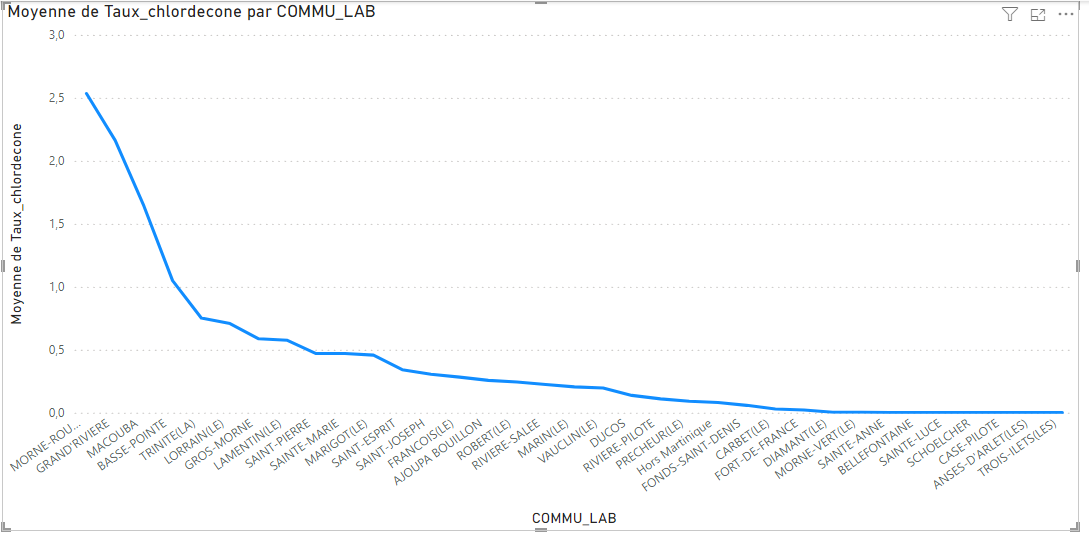
\includegraphics[width = 1
\linewidth]{moyenne_taux_chlordecone_par_commune.png}
\caption{Moyenne de Taux de Chlordécone par commune}
\end{figure}

\begin{figure}[!h]
\centering
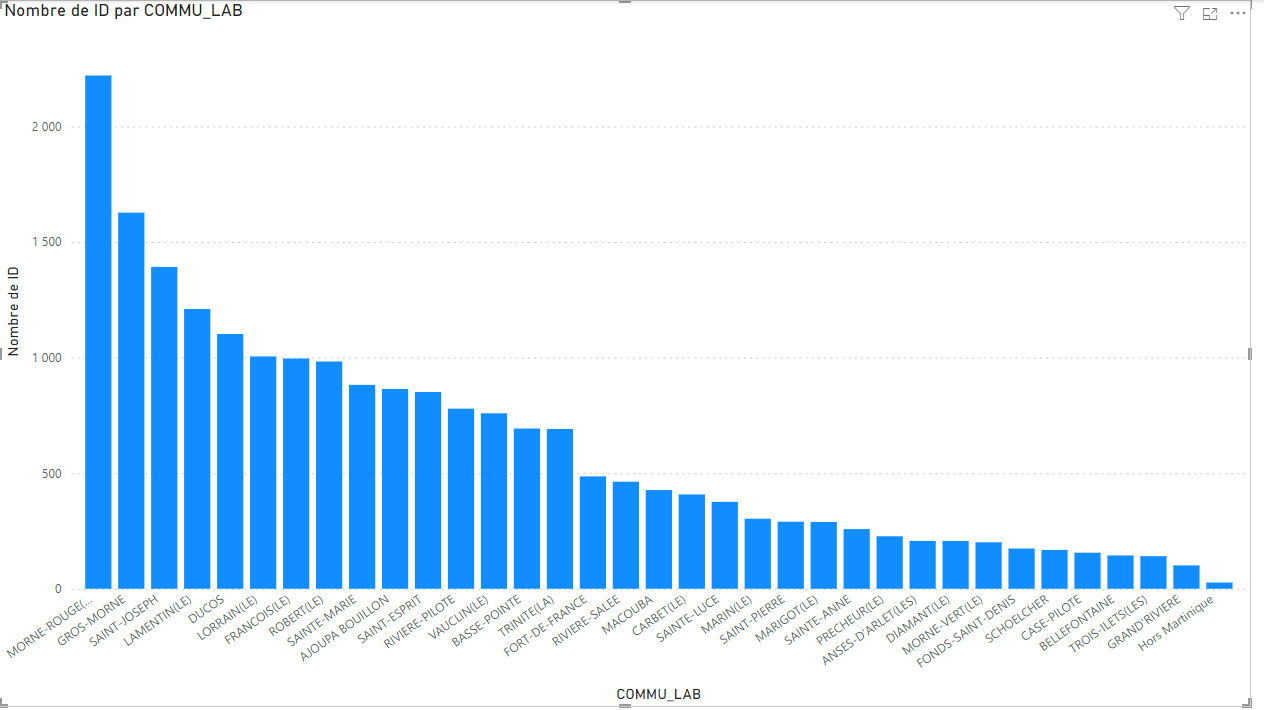
\includegraphics[width = 1
\linewidth]{nombre_prel_par_commune.png}
\caption{Nombre de prélèvement par commune}
\end{figure}

\textbf{Identification des tendances principales dans la dégradation du chlordécone et des facteurs environnementaux influençant ce processus.} \\ \\ 

Vérification de la normalité des résidus et  création d'un modèle de régression linéaire multiple avec les variables environnementales:\\  
Description du Modèle de Régression Linéaire Multiple\\
Objectif : Créer un modèle de régression linéaire multiple pour prédire le Taux de Chlordécone à partir de variables environnementales.\\

Variables :\\

Variable dépendante :\\

Taux\_chlordecone : La variable dépendante qu'on essaie de prédire.\\
Variables indépendantes :\\
moyenne\_pulviometrie : Moyenne des précipitations sur les sols.\\
mnt.exposition\_mean : Direction horizontale de la pente du terrain en degrés.\\
mnt.ombrage\_mean : Aspect des ombres du terrain.\\
mnt.pente\_mean : Inclinaison de la pente en degrés.\\
mnt.tpi\_mean : Indice de position topographique.\\

Sur le logiciel R on utilise les commandes qqnorm(resid(modele)) et qqline(resid(modele)) qui sont utilisées pour visualiser les résidus du modèle de régression. Elles créent un graphique Q-Q (quantile-quantile) qui permet d'évaluer si les résidus suivent une distribution normale. Voici le graphique:

\begin{figure}[!h]
\centering
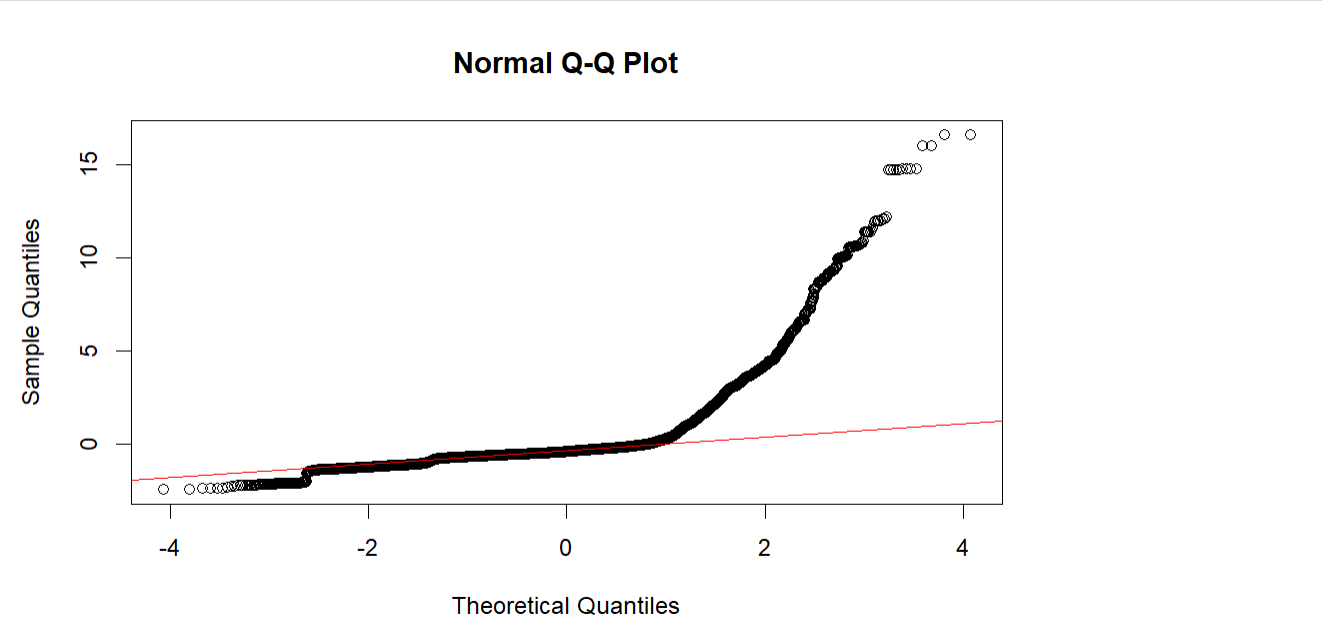
\includegraphics[width = 1
\linewidth]{graphiqueQQ.png}
\caption{Graphique Q-Q}
\end{figure}

Le graphique Q-Q (quantile-quantile) indique que les résidus ne sont pas normalement distribués. Les points qui dévient de manière significative de la ligne suggèrent que les résidus ne suivent pas une distribution normale. 
Cela peut signaler plusieurs problèmes potentiels, notamment :\\
Variabilité non constante (hétéroscédasticité) : Les variances des résidus peuvent ne pas être homogènes à travers les observations, ce qui viole une des hypothèses de base de la régression linéaire.\\
Les valeurs aberrantes peuvent déformer la distribution des résidus.\\





Ces déviations par rapport à la normalité des résidus peuvent affecter la validité des inférences statistiques dérivées du modèle. Il est donc important d'identifier et de traiter ces problèmes pour améliorer la qualité et la fiabilité du modèle.\\

A partir de ce modèle on a tracer l'histogramme des 



\end{document}
